\chapter{Extensive air shower parameters estimation}

\begin{figure}
	\label{pic:deconvolution-and-reconstruction}
	\centering
	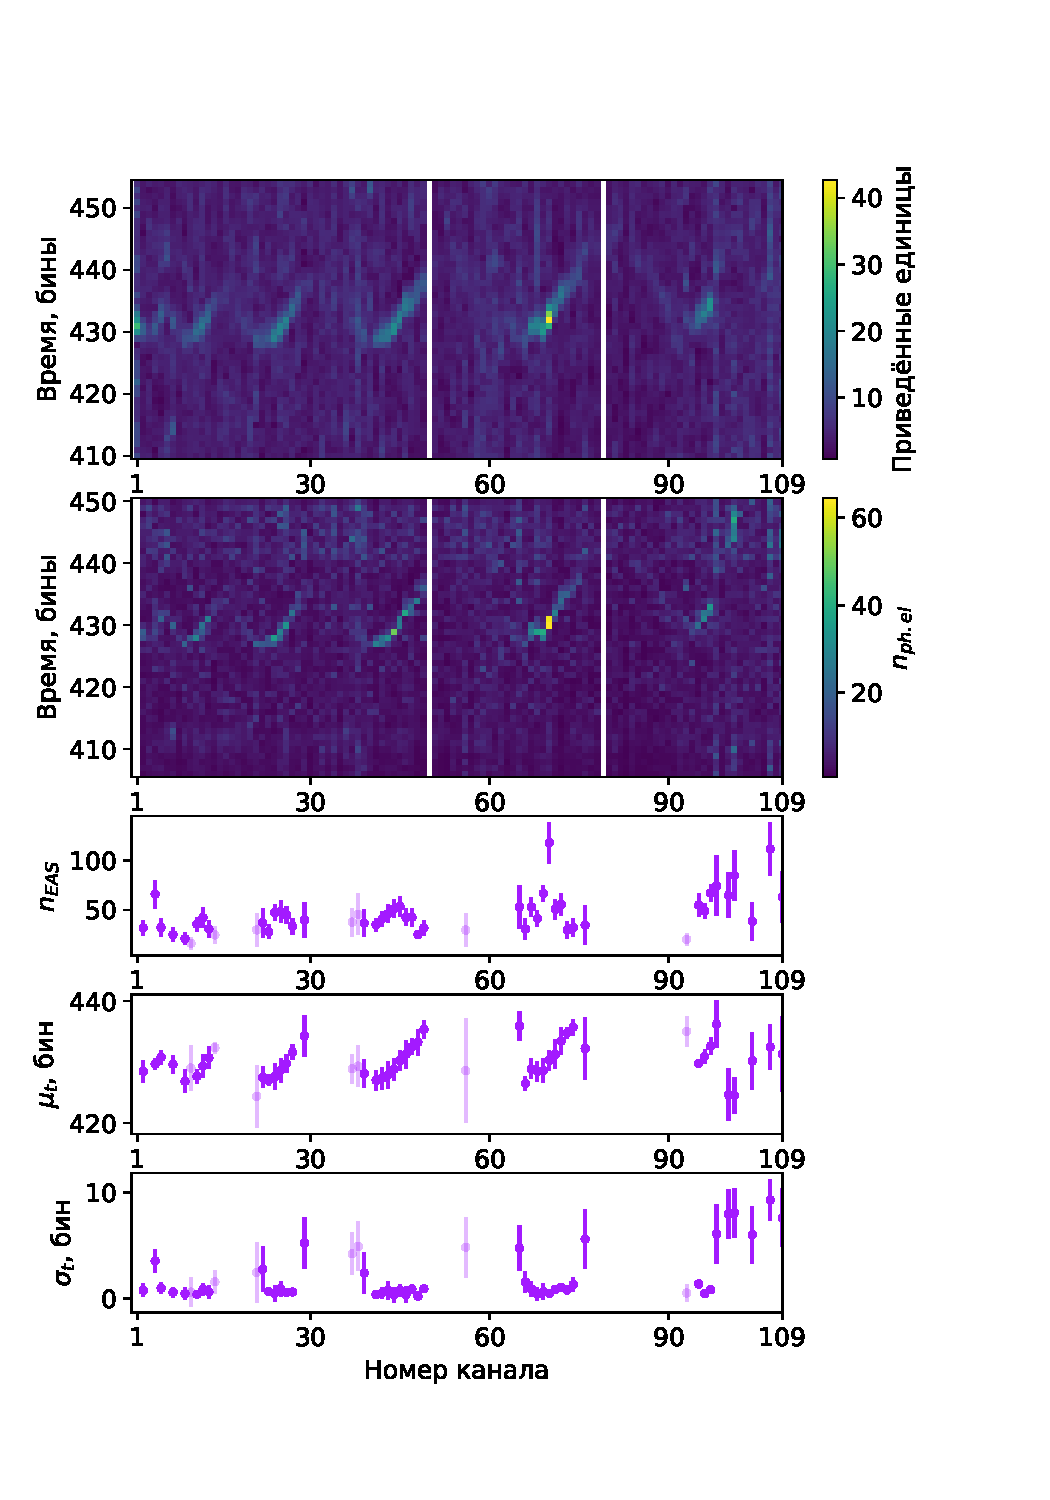
\includegraphics[width=0.83\columnwidth]{deconvolution-and-reconstruction}
	\caption{Full signal reconstruction for experimental event \#10675. Common X axis: channel number, see \cite{SphereCalibration2016} for numbering scheme. Top panel: experimental data with calibration coefficiens applied. Second-to-top panel: deconvolution output, photon count in each time bin. Three bottom panels: reconstructed photon packet parameters $n_{EAS}, \mu_t, \sigma_t$ --- dots and error bars represent marginal means and standard deviations; dimmed values are signals with $\Delta \mathrm{BIC} \in (0, 4]$, negative $\Delta \mathrm{BIC}$ (background-only channels) are omitted.}
\end{figure}

\section{Shower photon packets}
\label{sec:signal-reconstruction}

After deconvolution, we detect EAS photons among the background by searching for photon "packets" with a normal distribution of arrival times described by parameters $n_{EAS}$ (total photons), $\mu_t$ (mean arrival time), and $\sigma_t$ (arrival time standard deviation). The background comprises starlight and zodiacal light reflected from the snow, modeled as a Poisson distribution with a mean $\lambda_{n}$ known from calibration.

We approach this as a Bayesian problem, aiming to find the posterior distribution of photon packet parameters based on the distribution of $\vec{n}$ obtained from deconvolution. This is achieved using a similar MCMC technique. Performing both steps of the analysis within the same Bayesian framework lets us effectively chain these two analysis together, while also keeping them separate.

To assess the significance of the EAS signal in each channel and remove background-only channels from further analysis, we employ the Bayesian information criterion (BIC) \cite{Schwarz1978}.



Figure \ref{pic:deconvolution-and-reconstruction} presents an example illustrating the complete reconstruction of EAS photon packet parameters for an experimental event.

\section{Shower parameter reconstruction}

The rest of the reconstruction performed here in this work standard methods, with the exception of being applied to the output of Bayesian reconstruction.

\begin{itemize}
	\item \textbf{Shower arrival direction} is determined by a plain fit of arrival times. Ground level arrival times for each channel are determined from $\mu_t$ by subtracting ground-to-detector light travel time, accounting for the detector altitude and inclination.
	\item \textbf{Shower axis position} is determined by finding a point on the surface that maximizes the probability (with respect to each channel's posterior distribution) of monotonously decreasing lateral distribution function.
	\item \textbf{Lateral distribution function} for EAS Cherenkov light is determined by fitting a parametrized function to the data. In  this work, a simplified LDF from \cite{Budnev2005} is used. The fitting is done by convolving the LDF with each channel's light collection function (which is calculate from detector's optic system model). Shower energy is then derived from LDF parameters.
\end{itemize}
